\chapter{Memory}

\begin{center}
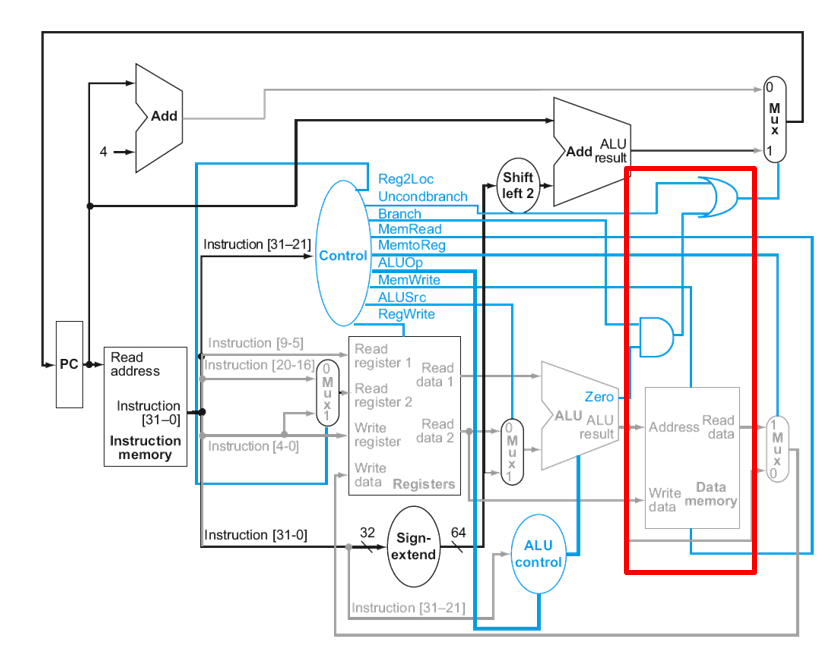
\includegraphics[width=5.5in]{../images/data_memory.png}
\end{center}

\section{Memory Stage}
Today we will create the iMemory stage of our processor.  This stage contains the data memory for the system that we use for load and store commands.  It also contains the logic gates used to produce the pc\_src signal that is used in the iFetch stage.  Note that although the diagram shows the pc\_src mux on the right side of the diagram, the mux is actually already implemented in the iFetch stage and belongs in the iFetch stage.

\section{Branch Resolution}

We now have all the information necessary to decide if the computer should branch or not.  We have the signal `branch' to tell us if it is a branch command, and we have `zero' to tell us if the condition was met.  Both branch and zero must be true so we will combine them with an `and' gate.

We also need an 'or' gate to 'or' together the output of the branch 'and' gate (above) and the uncondBranch control signal.  These gates can be included in your iMemory module as one line commands.  They do not need to be explicitly tested, as they will be thoroughly tested when we integrate the system.  

\section{Data Memory}

This will be similar to the register file memory, with two primary changes:
\begin{enumerate}
\item reading is now conditional on the MemRead control wire being high.  If the MemRead flag is not high, then the read\_data output should be set to Z (high impedance).
\item writing is now permissible if the MemWrite control wire is high.
\end{enumerate}
Create a data\_mem.v file, copy the contents of your register file memory and modify it to meet the needs of the data memory module.  You will also need to create a new data file, ramData.data that contains the initial values to be read into memory.

\section{Test Bench}
For this lab, we will just have a single test bench that will test the entire iMemory stage.  The test bench should verify the following:
\begin{enumerate}
	\item Correct logic for branching using the zero flag, branch control signal, and unconditional branch control signal
	\item That data can be read correctly from the iMemory module, verifying that you receive the correct value from ramData.data.
	\item That data can be written successfully to memory.  To verify that the write worked correctly, make sure to read from that address and verify that you read the updated value.  
\end{enumerate}


\section{Your Assignment}

You are to:
\begin{enumerate}
\item Create a new module called iMemory.
\item Instantiate the AND and OR gates directly in the iMemory stage.
\item Create a new module called data\_mem to handle data memory access.  Also create or modify a ramData.data file that contains initial values to be read into memory.
\item Integrate data\_mem into the iMemory stage.  
\item Write a testbench to verify that the iMemory stage works properly. 
\item Create a lab report in the LabN format.
\end{enumerate} 